\documentclass{standalone}
\usepackage{tikz}
\usepackage{amsmath}
\usepackage{bm}
\usepackage{pgfplots}
\usepackage{xcolor}
\usetikzlibrary{calc}
\usetikzlibrary{angles,quotes} % for pic
\usetikzlibrary{arrows.meta} % for arrow size
\usetikzlibrary{bending} % for arrow head angle

\pgfplotsset{compat=1.18}

\begin{document}

\colorlet{xcol}{blue!70!black}
\colorlet{xcol'}{xcol!50!red}
\colorlet{vcol}{green!45!black}
\colorlet{acol}{red!50!blue!80!black!80}
\colorlet{gcol}{green!60!black}
\colorlet{myred}{red!65!black}
\tikzstyle{force}=[->,myred,very thick,line cap=round]
\tikzset{>=latex} % for LaTeX arrow head

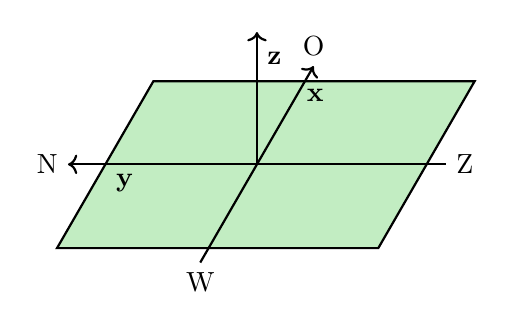
\begin{tikzpicture}[thick]
    \tikzset{arrowstyle/.style={->}}
    % conversion from cm to pt and vice versa
    \pgfmathsetmacro{\CmToPt}{28.3464566929}
    \pgfmathsetmacro{\PtToCm}{0.0352777778}
    

    \pgfmathsetmacro{\AxisSize}{2.4}
    \pgfmathsetmacro{\AngleAxes}{30}
    \pgfmathsetmacro{\AxesFactor}{0.6}
    % draw the tangent plane
    \pgfmathsetmacro{\RelPlaneSize}{0.85}
    \pgfmathsetmacro{\PlaneBound}{\AxisSize*\RelPlaneSize}        % extra boundary space around tangent plane
    \pgfmathsetmacro{\PlaneSize}{\AxisSize*2*\RelPlaneSize}         % extra boundary space around tangent plane
    \begin{scope}[xshift = (-\PlaneBound+sin(\AngleAxes)*\AxisSize*\AxesFactor)*\CmToPt, yshift= \PlaneBound * \CmToPt * cos(\AngleAxes) * \AxesFactor]
        \fill[green!70!black!60, opacity=0.4] (0, 0) -- (\PlaneSize, 0) -- ({\PlaneSize-sin(\AngleAxes)*\PlaneSize*\AxesFactor}, {-cos(\AngleAxes)*\PlaneSize*\AxesFactor}) -- ({-sin(\AngleAxes)*\PlaneSize*\AxesFactor}, {-cos(\AngleAxes)*\PlaneSize*\AxesFactor}) -- cycle;
        \draw (0, 0) -- (\PlaneSize, 0) -- ({\PlaneSize-sin(\AngleAxes)*\PlaneSize*\AxesFactor}, {-cos(\AngleAxes)*\PlaneSize*\AxesFactor}) -- ({-sin(\AngleAxes)*\PlaneSize*\AxesFactor}, {-cos(\AngleAxes)*\PlaneSize*\AxesFactor}) -- cycle;
    \end{scope}

    % draw the axes
    \draw[arrowstyle] (\AxisSize, 0) -- (-\AxisSize, 0)  node[pos=0.85, below] {$\mathbf{y}$} node[pos=1.0, left] {N} node[pos=0.0, right] {Z};
    \draw[arrowstyle] ({-sin(\AngleAxes)*\AxisSize*\AxesFactor}, {-cos(\AngleAxes)*\AxisSize*\AxesFactor}) -- ({sin(\AngleAxes)*\AxisSize*\AxesFactor}, {cos(\AngleAxes)*\AxisSize*\AxesFactor}) node[pos=0.85, right] {$\mathbf{x}$} node[pos=1.0, above] {O} node[pos=0.0, below] {W};
    \draw[arrowstyle] (0, 0) -- (0, \AxisSize*0.7) node[pos=0.8, right] {$\mathbf{z}$};



\end{tikzpicture}

\end{document}